%!TEX root = ../crimson_throne_book_main.tex
% 2015-10-03
While making their way to Palace Arkona, the companions worry about how to get inside. They have met Glorio Arkona once, but that might not be enough to broker an audience with the man. Upon approaching the compound our young heroes are marveled by its beauty. Black marble walls, topped with swirly iron decoration, line the grounds. An intricately forged gate allows a peek inside, revealing a magnificent marble palace with gold pillars, high windows and elegant minarets. The large, open garden hosts stylized bushes trimmed to look like elephants, opulent patches of imported trees and exotic flowers and fountains and statues depicting strange animals like tigers, apes, snakes and peacocks. Two guards stand inside the gate, but the companions' attention is immediately drawn to a third person walking up from the palace with a graceful stride. It is Selena, the Vudran beauty who was manipulating the uprisings in the city prior to the plague and who orchestrated the failed murder attempt on Aisha Leroung during the {\itshape Passion of Saint Alika} opera. She was also the one who alerted Balian to the threat at the Carowyn party, which allowed our heroes to take out the shadow creature before it killed off half of the city's noble youngsters. "At last you have arrived. My master has been expecting you. Please, follow me", she says as she opens the gate and leads the guests inside. She proceeds them up to the palace and through the front door, which is framed by a black marble arch depicting dozens of elephants standing atop each other.\hyperref[fig:Arkona-palace-in-Old-Korvosa-563928457]{ A rich hallway with a luxurious red carpet leads left and right, providing a pathway between several ebony doors. } Selena walks off to the right and rounds the corner to a corridor leading up to a fourteen-foot tall marble statue of a six-armed woman with four faces on her head, staring in every direction. Sjo is sure she represents a Vudran deity, but his knowledge of that pantheon is too limited to identify her. A door in the middle of the right-hand side of the corridor opens up into \hyperref[fig:Meeting-Glorio-Arkona-563929464]{ a comfortable lounge with a large fireplace and some snug sofas } . Lord Glorio Arkona is standing next to the hearth, with an impressive feline creature lying lazily at his feet. Spyder growls disagreeably as he sees the great tiger. Selena takes up her place between her master and a bare-chested man with broad shoulders, obviously a bodyguard. \\

\begin{figure}[h]
	\centering
	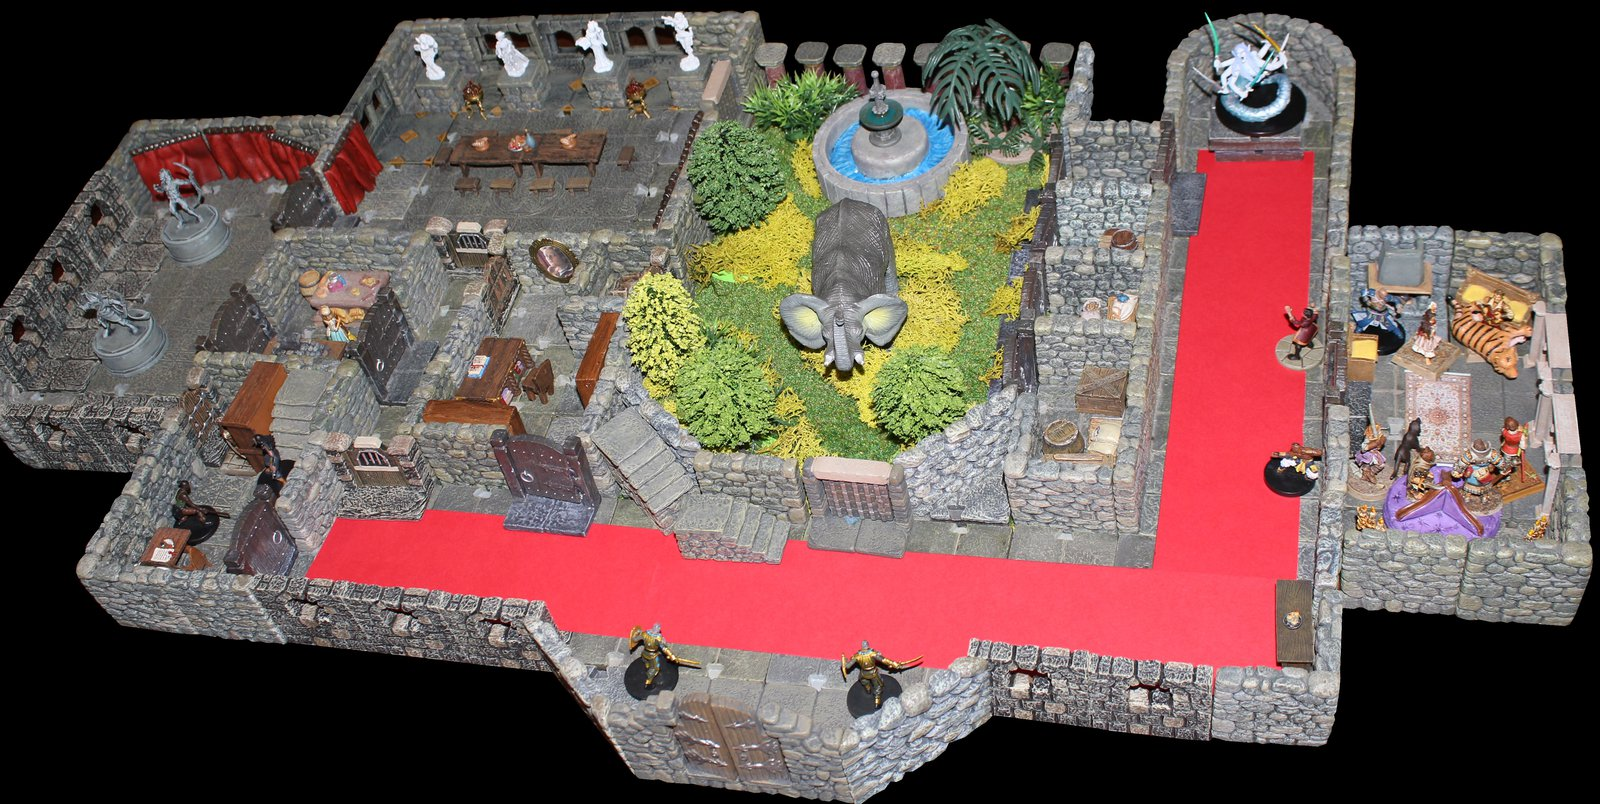
\includegraphics[width=0.39\textwidth]{images/Arkona-palace-in-Old-Korvosa-563928457.jpg}
	\caption{Arkona palace in Old Korvosa}
	\label{fig:Arkona-palace-in-Old-Korvosa-563928457}
\end{figure}

\begin{figure}[h]
	\centering
	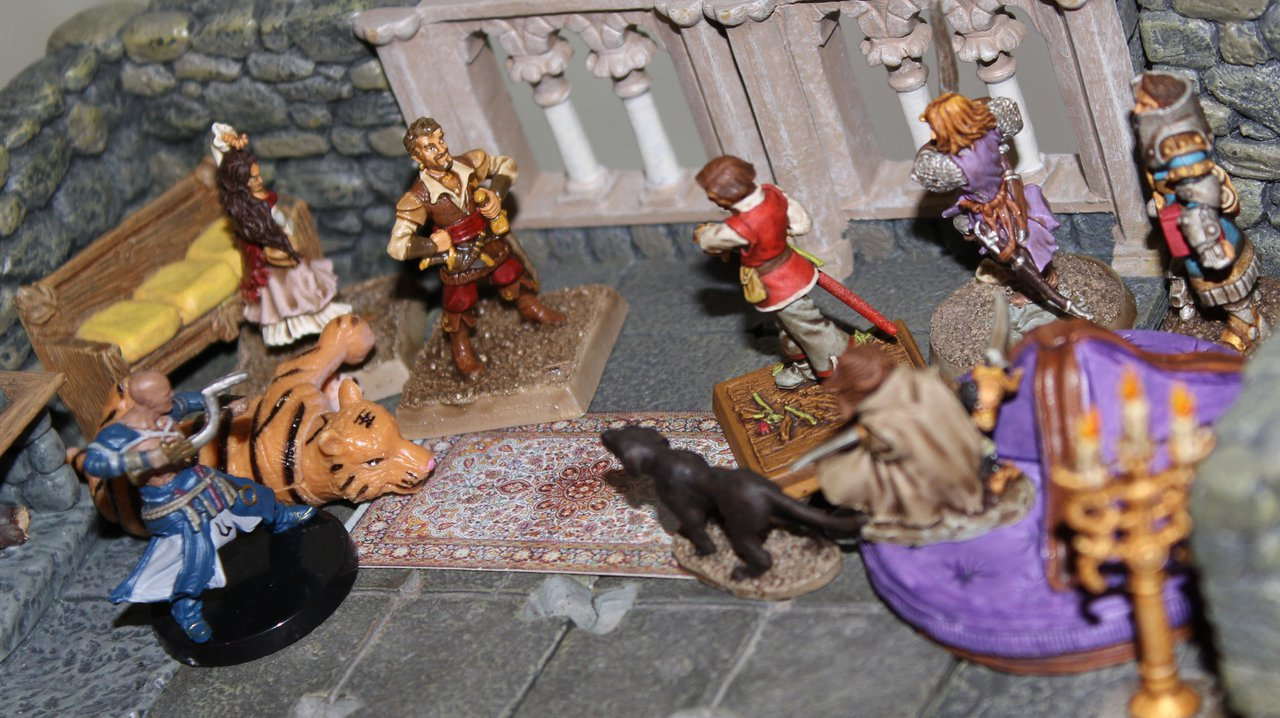
\includegraphics[width=0.39\textwidth]{images/Meeting-Glorio-Arkona-563929464.jpg}
	\caption{Meeting Glorio Arkona}
	\label{fig:Meeting-Glorio-Arkona-563929464}
\end{figure}

"Gentlemen," Glorio greets his guests, "it has been a while since last we met. A lot has occured in that time, wouldn't you say so? How are you doing? Can I offer you some refreshments, a glass of wine perhaps? Or would you prefer coffee and chocolate?"\\

While Selena leaves to get the refreshments, Lord Glorio bids his visitors to take a seat. He tells them he has been following their progress closely and appreciates the direction they have chosen recently. Quint immediately asks his host about seneschal Neolandus Kalepopolis and Vencarlo Orisini. Glorio wishes not to discuss them at this time, he states, as he wants to know first where the companions stand with regards to the queen. Lord Arkona makes no secret about having opposed the queen from the very start. He never trusted her, ever since she weaseled her way into king Eodred's bed years ago. Still, he tolerated her as long as the king was alive, but after Eodred's death, her malevolence became increasingly clear. She murdered her husband, got rid of the only person who had the authority to stop her - the senschal - and grabbed power in the city with no regard of its citizens.\\

Sjo objects to this analysis. He remains unconvinced of the queen's guilt, suspecting that she is being manipulated by an unseen power behind the throne. A likely suspect is her new seneschal, Magister Togomor. Lord Glorio smiles at Sjo's suspicions, but wipes them off the table: Togomor did not get involved until after the riots. Before that he was just doing his job in the Acadamae, while Ileosa was already plotting her evil. Sjo also refers to the {\itshape commune} that archbishop Keppira d'Bear of Pharasma performed. Although he agrees that most answers could possibly incriminate Ileosa, there was one question that supported Sjo's theory of a manipulative force behind the queen: the fact that she was being  {\itshape misled} by one of her advisors. Glorio rolls his eyes at this line of reasoning, saying that we are all being misled some way or another. Even the most insignificant effort to mislead Ileosa about the most pointless thing imaginable would have prompted a 'yes' from the commune question. Hardly any proof that the queen is someone else's puppet. Quint also points out that he and his friends met the queen before all the trouble started, when they returned her brooch to her. She was a different woman back then, sweet and innocent, not the ice-queen they saw when she killed commander Marcus Endrin of the Sable Company. Again Glorio nods and says this only supports his theory that the queen is evil and that they have to stop her. Sjo tries to meet his host halfway, by claiming that he does not stand {\itshape against} Ileosa, but  {\itshape for} Korvosa. He does agree that something has to be done about the  {\itshape castle} and Glorio seems to be satisfied with that. Now the Lord of House Arkona is willing to talk about Neolandus Kalepopolis and Vencarlo Orisini. He admits that Salvator Scream, the painter, brought the seneschal to him and that he aided the man by providing a safe place to hide. At Kalepopolis's own request - Glorio claims - he cannot reveal where that is yet. He does know where Vencarlo Orisini is, but fears that it is not in a good place.\\

The swordmaster is a respectable man, Glorio feels, who fights for the right cause as well, albeit mostly on his own, which explains his limited success. Anyway, in his search for the seneschal, Vencarlo Orisini followed up on Scream's hints and came to the Arkona Palace only three nights ago. Apparently the fencing master was a well-informed man as well, Arkona muses, as he knew about the secret dungeons under the palace. Orisini snuck in and did something quite unfortunate: he entered a place called the {\itshape vivified labyrinth} , wrongly suspecting that Kalepopolis would be in there. The labyrinth is some sort of deathtrap dungeon, Glorio sighs. It was constructed over two centuries ago by one of his forefathers, Eduardo Arkona. Glorio points to the painting of a handsome man above the fireplace: his face clearly shows several Vudran features, like a tanned skin and dark eyebrows. A bright red silk shawl covers his hair and completes the exotic look. Eduardo was Nerio Arkona's son, the man who established the trade route with Vudra and erected the family's palace in Korvosa. Eduardo completed his father's work by building the {\itshape vivified labyrinth} underneath, a place said to house  {\itshape Nerio's treasure} . None of the Arkona's, nor any of their Vudran servants have ever entered the labyrinth, as powerful magic keeps anyone with Vudran blood out. Nerio's descendants have repeatedly tried to send hired adventurers in and reclaim the treasure, but no one ever came out of the dreaded dungeon alive. Glorio's grandfather Horatio was the last to attempt such an enterprise, but Glorio's father Marco banned the practice and his son kept to the same rule. This implies that no one entered the vivified labyrinth for two generations, until Vencarlo stupidly decided to go in three nights ago. Glorio has no way of knowing if Vencarlo is still alive, but he wants to offer the companions the opportunity to find out, since Vencarlo is a friend of theirs who is worth saving and the man might make a capable ally in the struggle against the queen ... or castle. Glorio also admits that the 'treasure' intrigues him: it has been an unsolved mystery in his family for over two hundred years and who knows ... it might just be a powerful tool in their quest to help Korvosa. Glorio even offers the heroes a magic ring as payment, hoping the item can be of help inside the labyrinth. Sjo uses Zellara's cards to identity the piece of jewelry as a {\itshape ring of evasion} . 